\documentclass[runningheads]{llncs}

\usepackage[T1]{fontenc}
\usepackage{amsmath,amssymb,amsfonts}
\usepackage{algorithmic}
\usepackage{graphicx}
\usepackage{xcolor}
\usepackage{booktabs}
\usepackage{url}
\usepackage{array}
\usepackage{multirow}

\newcolumntype{L}[1]{>{\raggedright\arraybackslash}p{#1}}

\begin{document}

\title{A Drift-Aware MLOps Framework for Multi-Model Serving: A Network Intrusion Detection Case Study}

\titlerunning{A Drift-Aware MLOps Framework for Multi-Model Serving}

\author{Hoang Tran-Nguyen-Viet\inst{1} \and
Thai Bui-Ngoc\inst{1} \and
Tuan Le-Anh\inst{1} \and
Bao Nguyen-Van\inst{1} \and
Quan Le-Trung\inst{1}
}

\authorrunning{Hoang Tran-Nguyen-Viet et al.}

\institute{Faculty of Computer Networks and Communications,\\
University of Information Technology, VNU-HCM,\\Ho Chi Minh City, Vietnam\\
\email{\{23520541,23521412\}@gm.uit.edu.vn, \{tuanla,baonv,quanlt\}@uit.edu.vn}}

\maketitle

\begin{abstract}
Machine learning services can degrade when production data distributions change, even if source code remains unchanged. This issue is critical for network intrusion detection, where benign traffic and attack behavior evolve over time. This paper presents a baseline drift-aware MLOps framework for user-imported and training-job-created tabular models, using Network Intrusion Detection Systems (NIDS) as a case study rather than proposing a new classifier. The main contributions are threefold: a tenant-aware control-plane/data-plane architecture that separates model governance from online serving; a Native Registry abstraction that keeps model ownership, versions, deployability metadata, production-log summaries, drift results, and lifecycle state in PostgreSQL as the product-level source of truth; and a drift-aware lifecycle formulation connecting model onboarding, inference logs, production windows, drift scores, and review-driven actions. The prototype integrates Django/FastAPI services, Redpanda, Argo Workflows with Kubeflow PyTorchJob resources, S3-compatible storage, optional MLflow support, and Evidently AI. Preliminary NIDS experiments illustrate artifact onboarding, API serving, drift monitoring, offline recovery evaluation, and bounded replay observations without claiming production-scale performance.

\keywords{MLOps \and Data Drift \and Multi-model Serving \and Model Monitoring \and Network Intrusion Detection}
\end{abstract}

\section{Introduction}

Machine learning (ML) models are increasingly deployed as continuously running services rather than offline experimental artifacts. In a production setting, a model receives new input samples over time, generates predictions for downstream users or systems, and depends on monitoring mechanisms to remain trustworthy. Unlike traditional software services, an ML service may degrade even when its source code and infrastructure remain unchanged. One major cause is Data Drift, where the production data distribution differs from the reference distribution used during training, validation, or initial deployment.

This problem is especially relevant in Network Intrusion Detection Systems (NIDS). Network traffic is non-stationary: benign usage patterns change, infrastructure evolves, and attack strategies continuously adapt. A classifier trained on historical flow features may therefore become less reliable when deployed in a new environment or under a new attack distribution. An operational NIDS should not only expose a prediction API but also record production data, compare it with reference data, and trigger lifecycle actions when the monitored distribution changes.

Existing MLOps research provides architectural concepts for automating ML development, deployment, and monitoring \cite{kreuzberger2023mlops}. Other works discuss MLOps maturity, pipeline platforms, data quality, and continual model maintenance \cite{john2021towards,subramanya2022devops,renggli2021data}. However, practical systems often treat monitoring as a passive observability layer. In many prototypes, drift reports are generated after deployment, but the monitoring result is not explicitly modeled as a control signal for model lifecycle decisions.

This paper presents a baseline framework that connects multi-model serving with drift-aware monitoring. The goal is to describe a reusable MLOps framework, not to claim a new state-of-the-art NIDS classifier. In the proposed design, NIDS is used as a case study because it naturally exposes the need for drift-aware operation. The framework is intentionally scoped to tabular classification models that are either imported by users or produced by controlled training jobs and then converted into serving-compatible artifacts.

The main contributions of this paper are:

\begin{itemize}
    \item We propose a tenant-aware and drift-aware MLOps framework that integrates model onboarding, dynamic serving, production logging, drift detection, and lifecycle adaptation triggers.
    \item We formalize the framework using tenants, model functions, reference data, production windows, feature-level drift indicators, dataset-level drift ratio, and an action-selection function.
    \item We implement a prototype platform and instantiate it with a Network Intrusion Detection case study to demonstrate the feasibility of the proposed lifecycle.
\end{itemize}

The remainder of this article is structured as follows. Section~2 reviews related work on MLOps lifecycles, serving platforms, data quality, drift monitoring, and ML-based NIDS. Sections~3--5 define the problem, present the framework, and describe the drift-aware lifecycle algorithm; Sections~6--8 instantiate the framework in the NIDS case study, describe the prototype, and report preliminary evaluation results. Sections~9 and~10 discuss limitations and conclude the paper.

\section{Related Work}

MLOps extends DevOps principles to ML systems by coordinating data engineering, experimentation, training, deployment, monitoring, and governance. Kreuzberger \textit{et al.} define MLOps as a paradigm for reliably and efficiently maintaining ML systems in production \cite{kreuzberger2023mlops}; John \textit{et al.} propose an adoption maturity model \cite{john2021towards}; Sculley \textit{et al.} identify technical debt beyond model code, including data dependencies, configuration, monitoring, and feedback loops \cite{sculley2015debt}; and Amershi \textit{et al.} show that ML engineering differs from traditional software engineering because data, models, and code evolve together \cite{amershi2019software}. This paper narrows these lifecycle concerns to drift-aware signals for tenant-aware multi-model serving.

Platform studies provide complementary building blocks. TFX integrates ingestion, validation, training, and serving \cite{baylor2017tfx}; MLflow supports tracking and model lifecycle management \cite{mlflow}; and Clipper frames online prediction as a systems problem \cite{crankshaw2017clipper}. Pipeline and domain case studies \cite{zhou2020pipeline,subramanya2022devops}, self-adaptive MLOps architecture work \cite{Bhatt2025HarmonE}, and a recent empirical comparison of MLflow, Metaflow, Airflow, and Kubeflow Pipelines \cite{MarcosMercade2026MLOpsFrameworks} show complementary strengths rather than one universal lifecycle abstraction.

\begin{table}[t]
\caption{MLOps tool-family scope and remaining gap.}
\label{tab:mlops-tool-gap}
\centering
\small
\begin{tabular}{@{}L{2.2cm}L{3.2cm}L{5.8cm}@{}}
\toprule
\textbf{Tool family} & \textbf{Main support} & \textbf{Gap relative to this work} \\
\midrule
MLflow & Tracking, artifacts, registry. & Tenant ownership, lifecycle state, serving logs, and UI actions need product control-plane logic. \\
Flow tools & Workflow orchestration. & Registry governance, multi-model serving, and drift-driven review remain external concerns. \\
Kubeflow/TFX & Pipeline and cloud-native ML workflows. & Tenant lifecycle, registry views, and drift summaries must be mapped into application metadata. \\
Proposed framework & Registry, serving, logs, drift, and artifacts under one control plane. & Baseline prototype; production hardening and autonomous promotion remain future work. \\
\bottomrule
\end{tabular}
\end{table}

Production ML reliability depends on post-deployment data as well as the pipelines that manage it. Renggli \textit{et al.} treat data quality as a first-class MLOps concern \cite{renggli2021data}, and Polyzotis \textit{et al.} identify production data-management challenges \cite{polyzotis2017data}. Data Drift and concept drift are related but distinct: Gama \textit{et al.} survey adaptation to changing streams \cite{gama2014survey}, while Webb \textit{et al.} characterize forms of concept drift \cite{webb2016drift}. Here, Data Drift is an operational signal: because labels may be delayed or unavailable, the system first compares input distributions and then triggers inspection or workflow handoff.

Network intrusion detection is a non-stationary case study for this lifecycle. CIC-IDS2017 provides labeled intrusion traffic \cite{cicids}, but real environments can differ from dataset conditions. Sommer and Paxson highlight deployment context, generalization, and evolving traffic challenges for ML-based intrusion detection \cite{sommer2010closedworld}, and recent NIDS work treats concept drift as an operational problem requiring adaptation policies \cite{Zhang2025SSFNIDS}. This paper uses NIDS to illustrate lifecycle and monitoring requirements, not to claim a new state-of-the-art intrusion detection classifier.

The reviewed literature covers MLOps architectures, platforms, serving, data quality, drift adaptation, and NIDS deployment challenges. Existing tools provide useful building blocks, but they often center on tracking, orchestration, or pipeline execution rather than a tenant-facing lifecycle abstraction for multi-model serving. This paper addresses that gap by placing a Native Registry in the control plane as the product-level source of truth for tenant ownership, model families, versions, deployment metadata, production-log summaries, drift results, and review-driven lifecycle actions; the contribution is a control-plane integration pattern that owns lifecycle state while using existing tools as adapters.

\section{Problem Formulation}

Let $\mathcal{U}=\{u_1,u_2,\ldots,u_N\}$ denote the set of tenants using the platform. Each tenant $u \in \mathcal{U}$ owns a set of registered models:

\begin{equation}
\mathcal{M}_u=\{m_{u,1},m_{u,2},\ldots,m_{u,K_u}\}.
\end{equation}

Each model $m_{u,i}$ is represented by an inference function parameterized by $\theta$:

\begin{equation}
\hat{y}_t=f_{\theta}^{u,i}(x_t),
\end{equation}

where $x_t \in \mathbb{R}^{d}$ is the input vector at time $t$, $d$ is the number of input features, and $\hat{y}_t$ is the prediction. For a tabular classification model, $\hat{y}_t$ may be a class label or a probability vector over class labels.

For every inference request, the platform records a production log:

\begin{equation}
z_t=(u,i,x_t,\hat{y}_t,c_t,t),
\end{equation}

where $c_t$ is the prediction confidence if available. The log stream associated with a tenant-model pair $(u,i)$ forms the basis for monitoring.

Each deployed model has a reference dataset:

\begin{equation}
D_{\mathrm{ref}}^{u,i}=\{x_1,x_2,\ldots,x_n\},
\end{equation}

which represents the distribution observed during training, validation, or initial acceptance. At monitoring time $T$, the current production data window is:

\begin{equation}
D_{\mathrm{cur}}^{u,i}(T)=\{x_t \mid T-W \leq t \leq T\},
\end{equation}

where $W$ is the monitoring window size. The objective is not only to compute predictions but also to select a lifecycle action:

\begin{equation}
a_T = \pi(m_{u,i},D_{\mathrm{ref}}^{u,i},D_{\mathrm{cur}}^{u,i}(T),S_T),
\end{equation}

where $\pi(\cdot)$ is the adaptation policy and $S_T$ is the current lifecycle state of the model. Possible actions include no operation, alert generation, manual review, retraining review triggers, and candidate rollback or promotion records for human review.

For each feature $j$, the framework computes a drift score:

\begin{equation}
\delta_j=\Delta(P_{\mathrm{ref}}(x_j),P_{\mathrm{cur}}(x_j)),
\end{equation}

where $\Delta(\cdot)$ is a statistical distance or hypothesis test between the reference and current feature distributions. A feature-level drift indicator is defined as:

\begin{equation}
I_j =
\begin{cases}
1, & \delta_j > \tau_j,\\
0, & \mathrm{otherwise},
\end{cases}
\end{equation}

where $\tau_j$ is the threshold for feature $j$. The dataset-level drift ratio is:

\begin{equation}
\rho=\frac{1}{d}\sum_{j=1}^{d}I_j.
\end{equation}

The final drift decision is:

\begin{equation}
\mathrm{Drift}(D_{\mathrm{ref}}, D_{\mathrm{cur}}) =
\begin{cases}
1, & \rho \ge \tau_D,\\
0, & \text{otherwise}.
\end{cases}
\end{equation}

where $\tau_D$ is the dataset-level threshold. This formulation separates model prediction from monitoring and makes Data Drift an explicit input to lifecycle decisions.

\section{Proposed Framework}

The logical flow of the proposed framework consists of four stages. First, a user onboards a model artifact or registers an artifact produced by a controlled training workflow through the control plane. Second, the data plane exposes the model as a prediction endpoint. Third, each prediction produces an asynchronous log event. Fourth, the monitoring layer periodically reconstructs the current production window and compares it with the reference data. If drift is detected, the adaptation layer creates an alert or triggers a retraining review workflow.


\subsection{Control Plane}

The control plane manages user-facing and governance operations. It stores tenants, authentication credentials, API keys, model metadata, artifact locations, endpoint URLs, access modes, and model statuses. In the prototype, this layer is implemented using Django. A model record contains the model name, description, owner tenant, artifact URI, access mode, generated endpoint, and lifecycle status.

When a model artifact is uploaded or registered from a completed training job, the control plane validates the available metadata, stores artifact references, and records the model in the native registry. The model can then be assigned an endpoint of the form \texttt{/models/\{model\_id\}/predict}. This design decouples model ownership and metadata management from online inference.

\subsection{Data Plane}

The data plane is implemented as a generic FastAPI model server. The logical serving path resolves models through a shared API, while deployment adapters may create dedicated runtime resources when configured. The server reads the corresponding model metadata, loads the model artifact through MLflow pyfunc, validates the request payload against the expected input format when possible, and returns the prediction result.

Tenant-aware access control is enforced before inference. Public models can be invoked directly, while private models require a valid API key or bearer token. The resolved tenant identifier must match the model owner. This mechanism supports a platform setting where multiple users upload and serve independent models through a shared serving layer.

\subsection{Production Logging Layer}

Online inference should not depend synchronously on database writes. Therefore, the framework decouples prediction from logging through a message broker. After producing a prediction, the model server emits a production log event to Redpanda. A consumer service batches log events and persists them to PostgreSQL. Each log stores the tenant identifier, model identifier, timestamp, feature payload, and prediction result.

This design has two advantages. First, it keeps monitoring writes outside the synchronous prediction path. Second, it creates a unified production data source that can be queried per tenant and per model for drift detection, audit, and evaluation.

\subsection{Drift Monitoring Layer}

The monitoring layer compares reference data with recent production data. In the prototype, Evidently AI is used to compute feature-level drift and dataset-level drift summaries. Reference data can be stored as object storage artifacts, while production data are reconstructed from PostgreSQL logs. Drift reports can be exported as HTML or JSON artifacts for inspection.

\subsection{Adaptation Layer}

The adaptation layer maps monitoring outputs to lifecycle actions. In the baseline implementation, the primary action is a drift alert or workflow trigger. The framework can be extended to support retraining jobs, model evaluation gates, review-driven promotion, rollback, and notification workflows. This distinction is important: the current prototype demonstrates a drift-aware control loop, while fully autonomous retraining and deployment remain future work.

Figures~\ref{alg:onboarding} and~\ref{alg:monitoring} summarize the framework-level onboarding and drift-aware monitoring procedures.

\begin{figure}[t]
\small
\begin{algorithmic}[1]
\REQUIRE Model package or training artifact $A$, metadata $H$, tenant $u$
\ENSURE Registered model endpoint $e$
\STATE Validate package extension and archive structure
\STATE Validate serving metadata or record deployability status
\STATE Store or reference $A$ in artifact storage
\STATE Create model record $m_{u,i}$ in the control plane
\STATE Assign lifecycle state $S \leftarrow \mathrm{validated}$
\STATE Generate endpoint $e \leftarrow$ \texttt{/models/\{i\}/predict}
\STATE Return endpoint $e$
\end{algorithmic}
\caption{Model onboarding procedure.}
\label{alg:onboarding}
\end{figure}

\begin{figure}[t]
\small
\begin{algorithmic}[1]
\REQUIRE Input $x_t$, model identifier $i$, credential $q$
\ENSURE Prediction $\hat{y}_t$ and optional lifecycle action $a_T$
\STATE Authenticate $q$ and resolve tenant $u$
\STATE Retrieve model metadata $m_{u,i}$
\STATE Load or reuse cached model $f_{\theta}^{u,i}$
\STATE Compute prediction $\hat{y}_t \leftarrow f_{\theta}^{u,i}(x_t)$
\STATE Emit log event $z_t=(u,i,x_t,\hat{y}_t,t)$
\IF{monitoring condition is satisfied}
    \STATE Build production window $D_{\mathrm{cur}}^{u,i}(T)$
    \FOR{each feature $j=1$ to $d$}
        \STATE Compute drift score $\delta_j$
        \STATE Compute indicator $I_j$
    \ENDFOR
    \STATE Compute drift ratio $\rho$
    \STATE Select action $a_T \leftarrow \pi(m_{u,i},D_{\mathrm{ref}},D_{\mathrm{cur}},S_T)$
    \IF{$\rho \geq \tau_D$}
        \STATE Trigger alert, review, or workflow handoff
    \ENDIF
\ENDIF
\STATE Return $\hat{y}_t$
\end{algorithmic}
\caption{Drift-aware inference and monitoring procedure.}
\label{alg:monitoring}
\end{figure}

\section{Drift-Aware Lifecycle Algorithm}

The model lifecycle can be represented as a state transition system:

\begin{equation}
\begin{split}
S \in \{&
\mathrm{uploaded},\ \mathrm{validated},\ \mathrm{deployed},\
\mathrm{monitored},\\
&\mathrm{drifted},\ \mathrm{reviewing},\ \mathrm{retraining},\
\mathrm{promoted},\ \mathrm{failed}
\}.
\end{split}
\end{equation}

The transition function is:

\begin{equation}
S_{T+1}=\Phi(S_T,m_{u,i},\rho,\tau_D,a_T),
\end{equation}

where $\Phi(\cdot)$ updates the model state according to the drift ratio and the selected action. If $\rho < \tau_D$, the model remains in the monitored state. If $\rho \geq \tau_D$, the model is marked as drifted and the system can trigger alerting, review, or a workflow handoff.

\section{Case Study: Network Intrusion Detection}

The NIDS model is used as a case study to instantiate the proposed framework. A network flow is represented as a tabular feature vector $x \in \mathbb{R}^{d}$ containing statistics such as duration, packet counts, byte rates, and protocol-related attributes. The model predicts whether the observed traffic is benign or belongs to an attack class.

In the current prototype, XGBoost is selected as the baseline classifier rather than as a claim of state-of-the-art NIDS performance. The case study uses tabular network-flow features, where tree-based gradient boosting provides a practical balance between non-linear feature interaction modeling, training cost, inference efficiency, and artifact portability \cite{xgboost}. Compared with simple linear baselines, XGBoost can capture interactions among flow statistics such as duration, packet counts, and byte rates. Compared with deep neural models, it requires less task-specific architecture design and is easier to package, version, and serve as a compact artifact in a multi-tenant MLOps prototype. Therefore, XGBoost is used to exercise the lifecycle--training, packaging, registration, endpoint invocation, production logging, and drift monitoring--rather than to optimize NIDS classification accuracy. Other classifiers can be onboarded through the same artifact and registry workflow when they satisfy the serving contract.

NIDS is an appropriate case study for drift-aware MLOps for three reasons. First, network environments change over time, causing benign traffic distributions to shift. Second, attack patterns evolve, making historical training data incomplete. Third, labeled production data are often delayed or unavailable, so input distribution monitoring can provide an early warning signal before supervised performance metrics are available.

\section{Prototype Implementation}

The prototype uses a control-plane/data-plane split: the Django/DRF control plane stores tenant, job, registry, deployment, and drift metadata in PostgreSQL, while the FastAPI data plane resolves endpoints, loads artifacts, and emits log events for drift analysis. Table~\ref{tab:implementation} summarizes the implemented modules.

Figure~\ref{fig:prototype-flow} summarizes the implemented prototype workflow across the control plane, data plane, training execution, artifact storage, production logging, and drift monitoring components.

\begin{figure}[t]
\centering

\includegraphics[width=0.8\linewidth]{assets/flow.png}
\caption{Prototype workflow of the drift-aware MLOps framework. The Django control plane coordinates upload, packaging, training requests, deployment requests, registry metadata, and drift checks. The FastAPI data plane serves model predictions and emits production logs through Redpanda/PostgreSQL, while Argo/Kubeflow, object storage, Harbor, MLflow, Evidently, and Karpenter-backed compute are used as supporting services where configured.}
\label{fig:prototype-flow}
\end{figure}


\begin{table}[htbp]
\caption{Prototype modules and responsibilities.}
\label{tab:implementation}
\centering
\small
\begin{tabular}{@{}L{2.6cm}L{2.8cm}L{6.0cm}@{}}
\toprule
\textbf{Module} & \textbf{Implementation} & \textbf{Responsibility} \\
\midrule
Control plane & Django/DRF & Manages tenants, jobs, registry, deployment, and drift APIs. \\
Training execution & Argo/Kubeflow + runner & Executes configured entry points and returns artifacts. \\
Artifact/registry layer & Object storage + PostgreSQL & Stores model artifacts, metadata, and version summaries. \\
Packaging/serving & Packager + FastAPI & Prepares or loads serving artifacts and exposes prediction endpoints. \\
Logging/drift & Redpanda + consumer + Evidently & Persists production logs and stores drift summaries. \\
Deployment configuration & Docker Compose/K8s/Argo files & Supports local integration and prototype/testbed deployment. \\
\bottomrule
\end{tabular}
\end{table}
\begin{figure}[htbp]
\centering
\begin{minipage}[t]{0.49\linewidth}
  \centering
  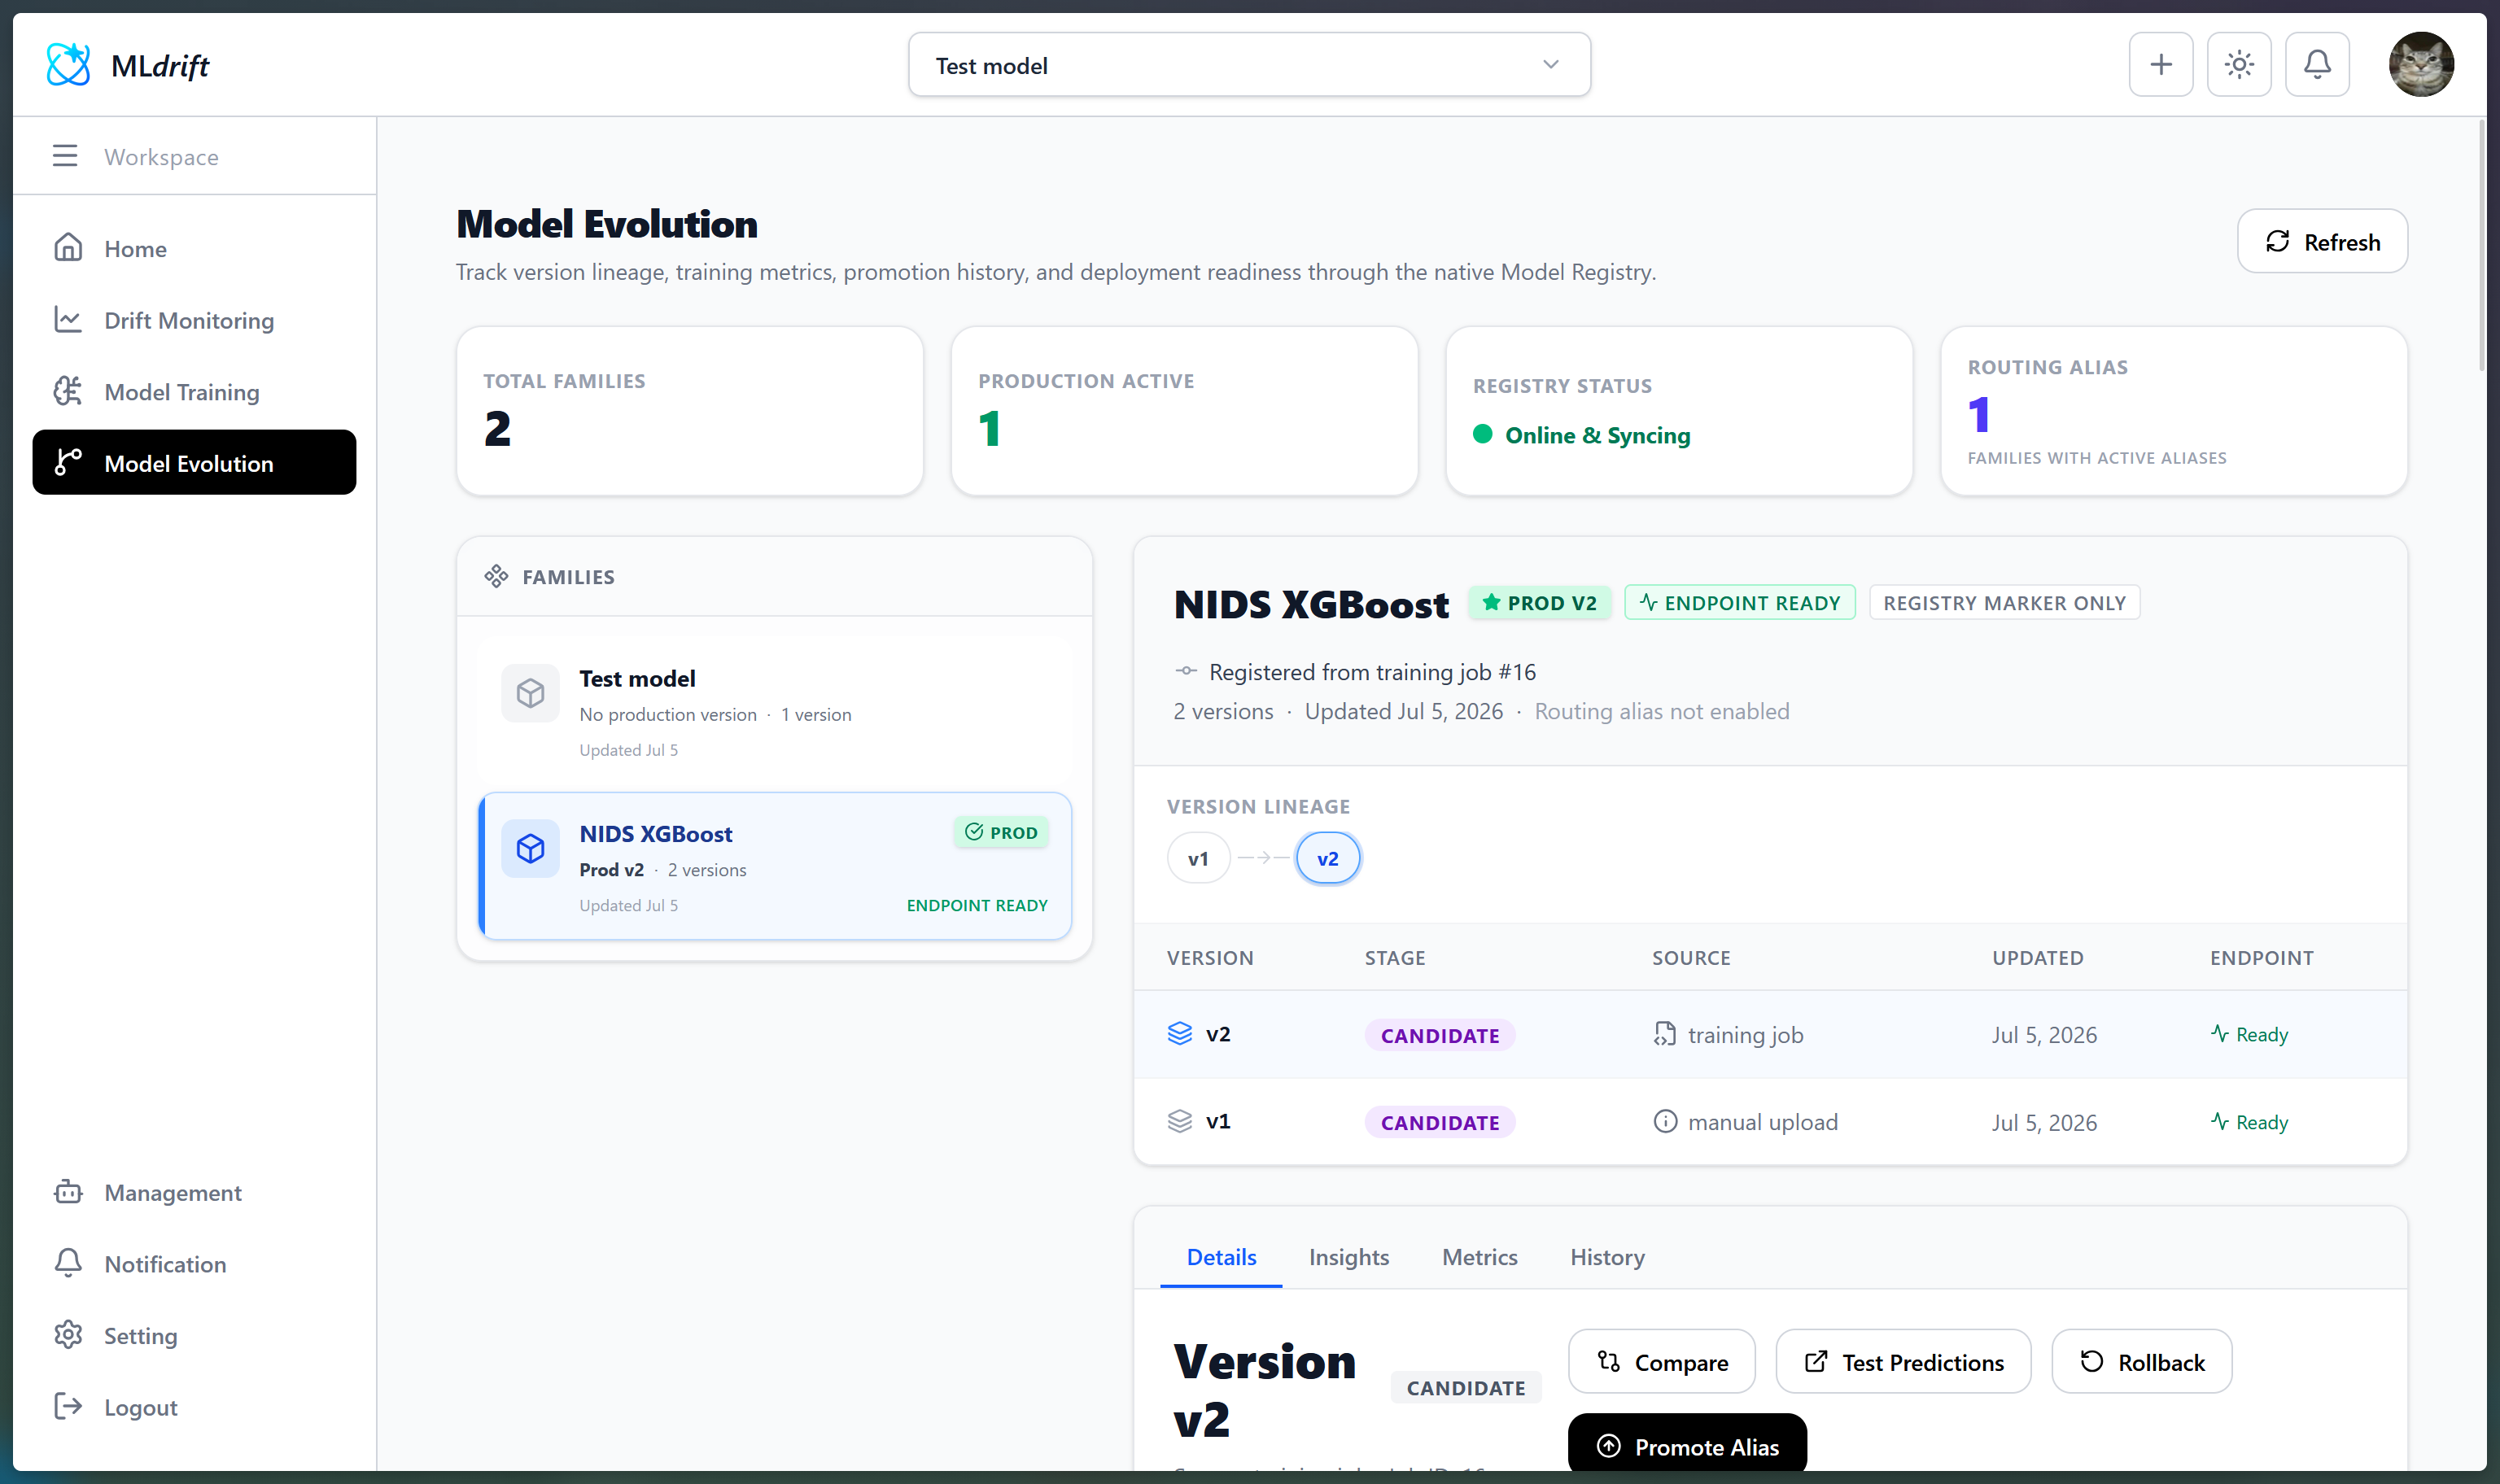
\includegraphics[width=\linewidth]{screenshots/10_model_evolution_v1_v2_lineage.png}
  \caption{Model Evolution UI showing version lineage (v1 $\rightarrow$ v2) and dynamic serving readiness.}
  \label{fig:ui-evolution}
\end{minipage}\hfill
\begin{minipage}[t]{0.49\linewidth}
  \centering
  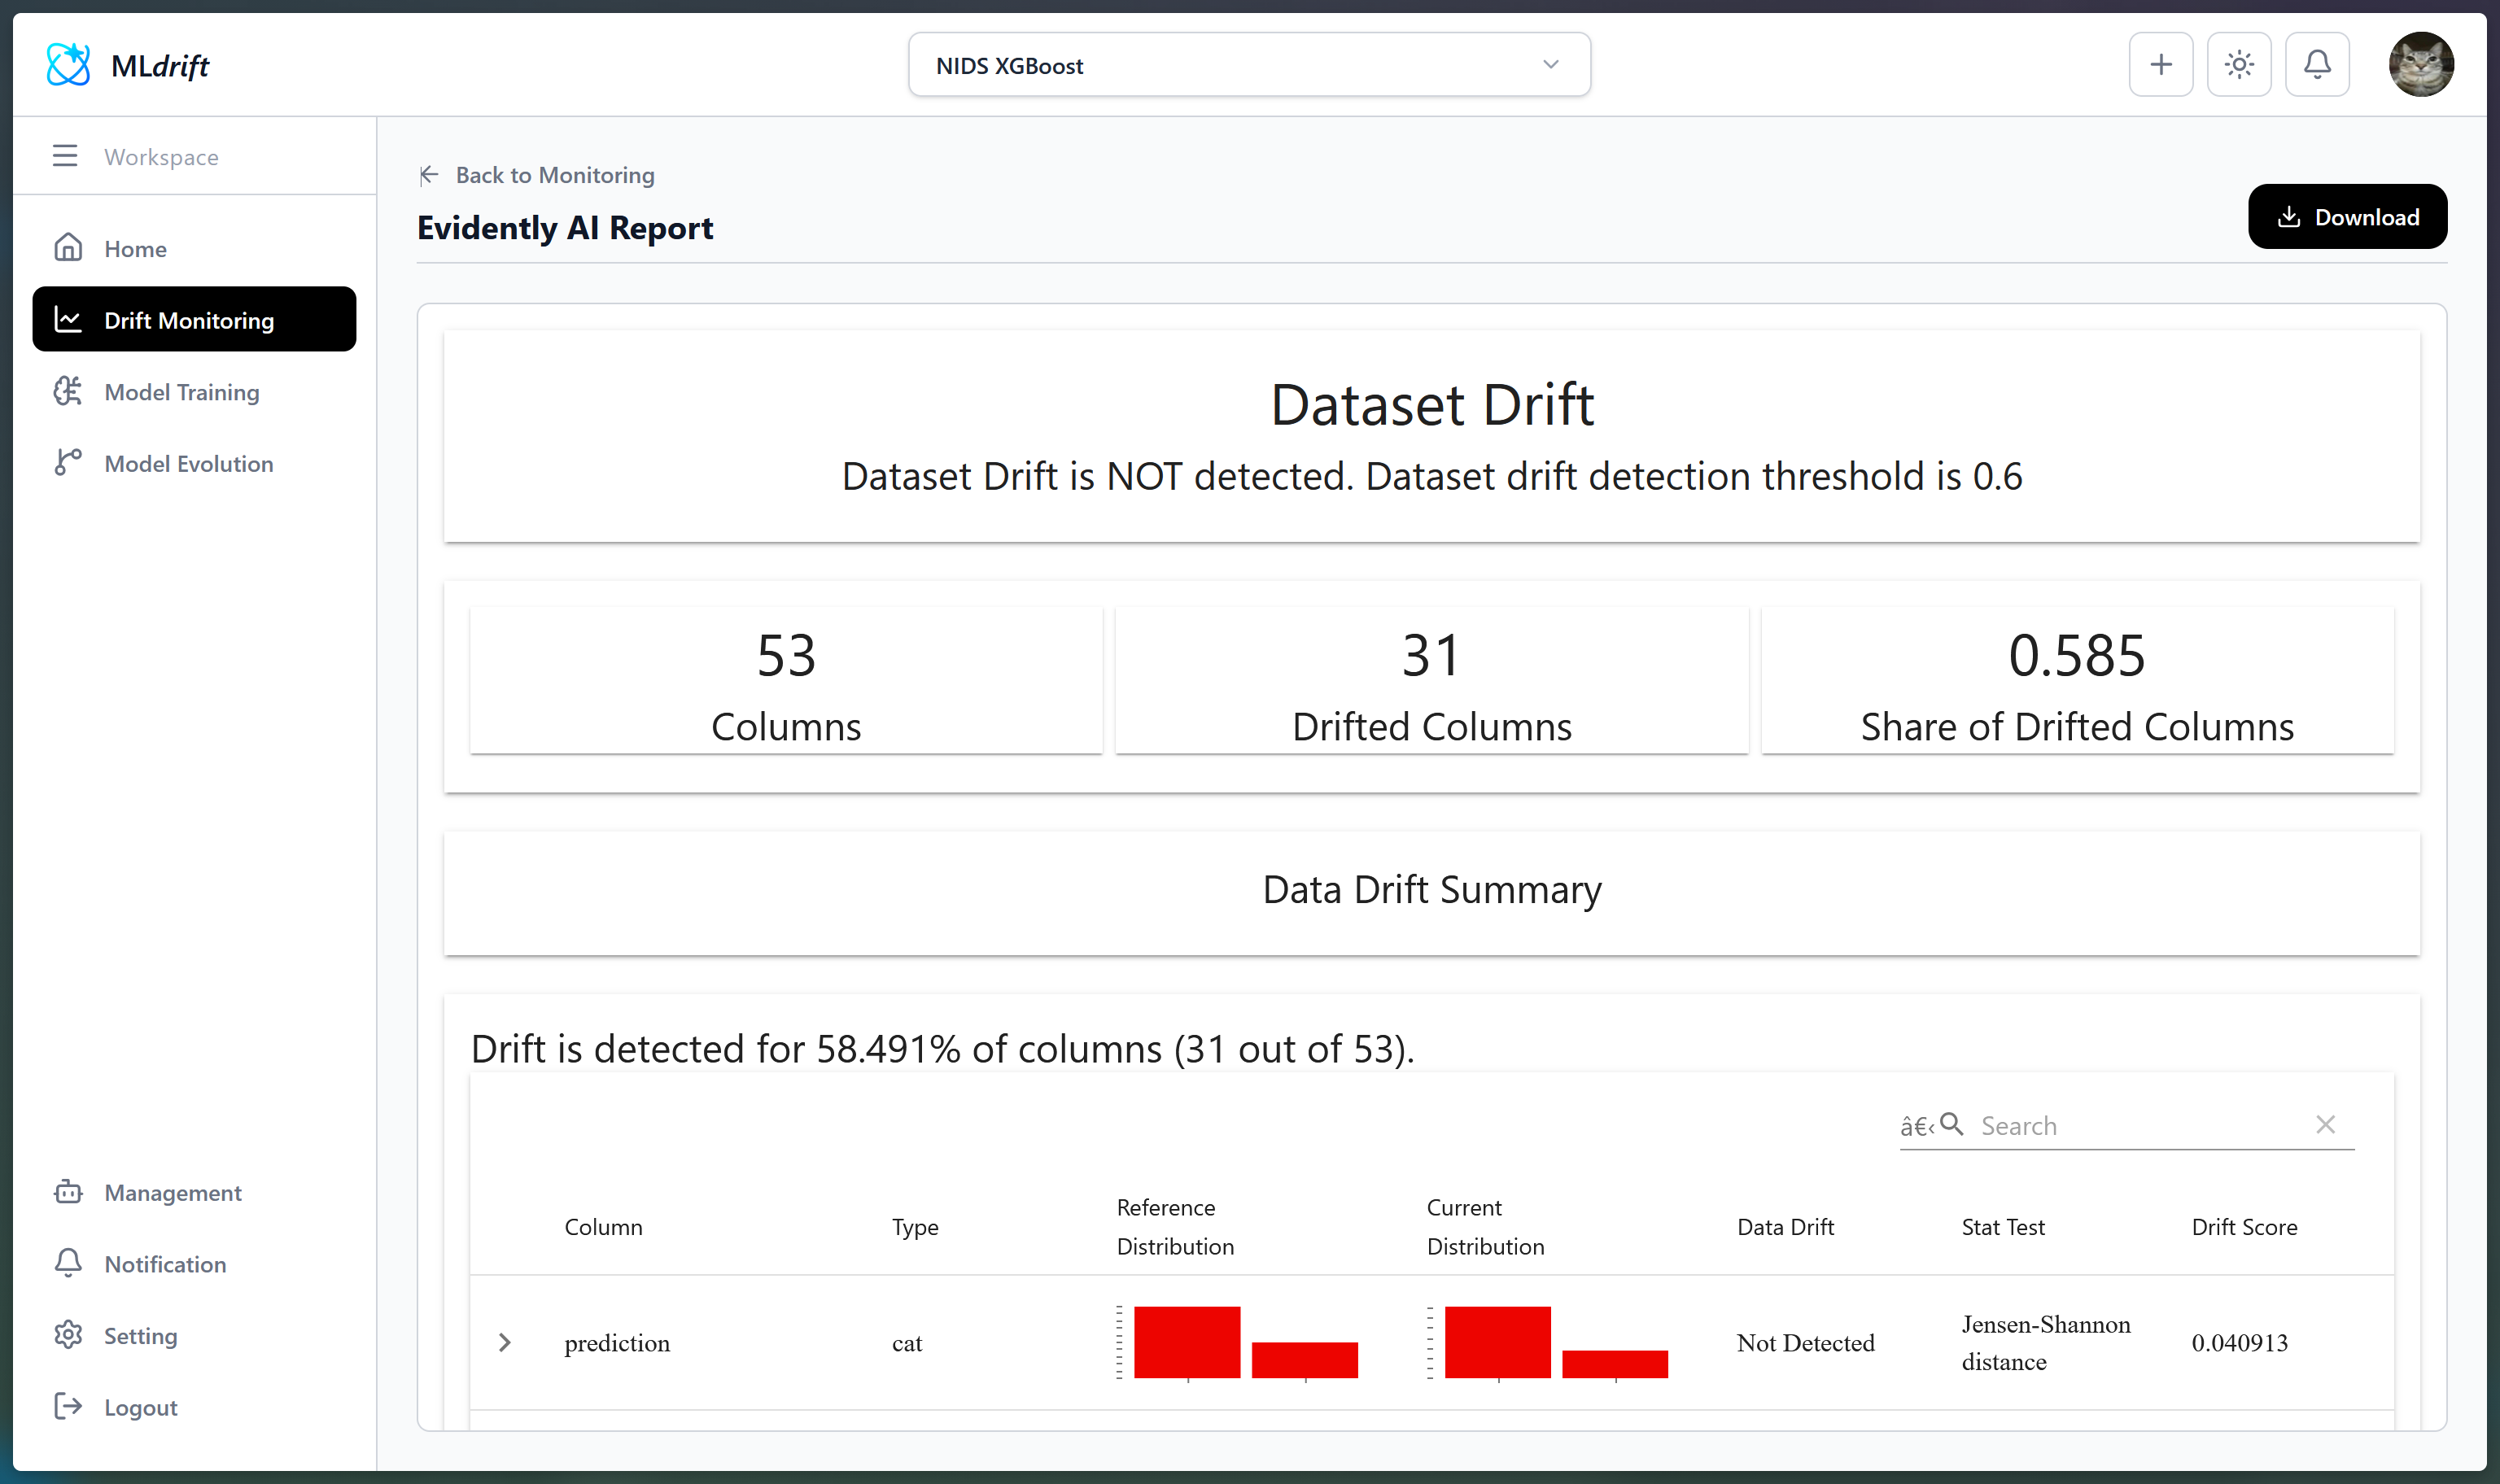
\includegraphics[width=\linewidth]{screenshots/14_drift_evidently_report_results.png}
  \caption{Evidently AI drift monitoring dashboard showing feature-level drift detection.}
  \label{fig:ui-drift}
\end{minipage}
\end{figure}

\textit{Training execution.} The control plane validates source code and reference data, submits a training webhook to Argo Events, and Argo Workflows instantiate a Kubeflow \texttt{PyTorchJob} on Karpenter-provisioned nodes. The runner executes the configured entry point, uploads the resulting \texttt{model.tar.gz} to S3, and a completion webhook ingests the artifact. User scripts do not need to import MLflow; an optional \texttt{\_mlops} bundle may include training metrics and a manifest, but its absence does not invalidate the artifact.

\textit{Metadata and registry.} When a completed job is ingested, the control plane extracts metrics, parameters, insights, and deployability summaries, which are mirrored into Model Evolution upon registration. The Native Registry links immutable model versions to tenant-scoped model projects, using PostgreSQL as the source of truth for ownership, lifecycle, and drift results. Figure~\ref{fig:ui-evolution} depicts the Model Evolution UI for the NIDS XGBoost family, illustrating version lineage from v1 to v2 with live serving readiness.

\textit{Packaging, serving, and monitoring.} The packager builds serving-compatible images via Argo and Docker, pushes them to Harbor, and creates a FastAPI pod exposing a prediction endpoint. Prediction logs flow asynchronously via Redpanda to PostgreSQL. Evidently computes drift reports on production windows; drift is an adaptation signal requiring human review without automatic redeployment. Figure~\ref{fig:ui-drift} illustrates the Evidently AI dashboard, where feature distribution shifts are evaluated via Wasserstein and Jensen--Shannon distances.

\textit{Deployment and operational scope.} The repository includes Docker Compose, Kubernetes (K3s) manifests, and Argo workflow templates for prototype and testbed deployment; where Karpenter is configured, training pods scale on AWS-backed GPU and CPU node pools on demand. The implemented baseline covers training, registry, serving, production logging, drift reports, and a basic routing alias; autonomous promotion, canary deployment, and production-grade hardening remain future work.

\section{Preliminary Evaluation}

Because this paper is a baseline, evaluation focuses on prototype feasibility and drift-aware lifecycle behavior rather than optimizing NIDS accuracy. We design an offline multi-level replay experiment on CIC-IDS2017-style binary BENIGN-vs-ATTACK data. For each attack family (PortScan, BruteForce, WebAttacks), the attack data are split into a trigger/retraining subset (60\%) and a future holdout subset (40\%). A production/drift window is constructed by mixing ATTACK rows from the future holdout with BENIGN rows at three controlled attack fractions: Mild ($\approx$15\%), Moderate ($\approx$40\%), and Severe ($\approx$85\%), producing nine evaluation points across a realistic range of distribution shift intensities. The framework-assisted path treats the drift decision as an alert initiating review-driven challenger retraining; it does not bypass review gates or perform automatic promotion. Row-hash checks prevent data leakage in all scenarios.

Drift is measured using the Kolmogorov--Smirnov (KS) test at $p < 0.05$ over 52 flow features. We report the \emph{mean KS statistic} as a continuous drift magnitude indicator. Figure~\ref{fig:ui-drift} illustrates a representative Evidently AI drift report generated by the monitoring layer. Table~\ref{tab:drift-multilevel} summarizes the results.


\begin{table}[htbp]
\centering
\caption{Multi-level drift recovery results. Atk\% = attack fraction in drift window. Mean KS = mean KS statistic across 52 features. $\Delta$M-F1 = Retrained M-F1 $-$ Fixed M-F1.}
\label{tab:drift-multilevel}
\small
\setlength{\tabcolsep}{4pt}
\begin{tabular}{@{}llccccc@{}}
\toprule
Attack Family & Level & Atk\% & Mean KS & Fixed M-F1 & Retrained M-F1 & $\Delta$M-F1 \\
\midrule
\multirow{3}{*}{PortScan}
  & Mild     & 17\% & 0.101 & 0.453 & 0.999 & +0.547 \\
  & Moderate & 40\% & 0.234 & 0.375 & 1.000 & +0.625 \\
  & Severe   & 85\% & 0.493 & 0.130 & 1.000 & +0.869 \\
\midrule
\multirow{3}{*}{BruteForce}
  & Mild     & 15\% & 0.068 & 0.460 & 1.000 & +0.540 \\
  & Moderate & 40\% & 0.181 & 0.375 & 1.000 & +0.625 \\
  & Severe   & 85\% & 0.386 & 0.131 & 1.000 & +0.869 \\
\midrule
\multirow{3}{*}{WebAttacks}
  & Mild     & 15\% & 0.085 & 0.460 & 0.997 & +0.538 \\
  & Moderate & 40\% & 0.224 & 0.375 & 0.996 & +0.621 \\
  & Severe   & 85\% & 0.482 & 0.130 & 0.983 & +0.853 \\
\bottomrule
\end{tabular}
\end{table}

The results show a consistent trend across all three attack families: as the attack fraction increases from Mild to Severe, the mean KS statistic rises from 0.07--0.10 to 0.39--0.49, and the fixed model Macro-F1 degrades from $\approx$0.46 to $\approx$0.13. Drift alerts are triggered in all nine scenarios, and retrained challengers recover Macro-F1 to 0.983--1.000, with $\Delta$M-F1 increasing with severity (+0.54, +0.62, +0.85--0.87). The high fraction of drifted features (51--52 of 52) reflects the controlled lab nature of CIC-IDS2017, where attacks produce highly discriminative flow patterns. In real-world deployments with more gradual shifts, the drifted-feature fraction would typically be 0.3--0.6. Results are presented as prototype feasibility evidence rather than production performance claims.

We also ran a bounded prototype serving replay against a testbed endpoint using Locust traffic and Prometheus metrics scraped from the serving pod. The 100-user run issued 4,343 client-side prediction requests over approximately 89 seconds. Locust observed an average request rate of 47.6 requests/s, an average response time of 1.74 s, p95 2.30 s, and four HTTP 502 responses. Prometheus reported a peak server-side rate of 144.1 requests/s and 1.60 s average handler latency. These observations indicate the prototype handled most requests but showed gateway errors under load. No SLA or production performance claim is made. Figure~\ref{fig:endpoint-benchmark} shows the Locust time series.

\begin{figure}[t]
\centering
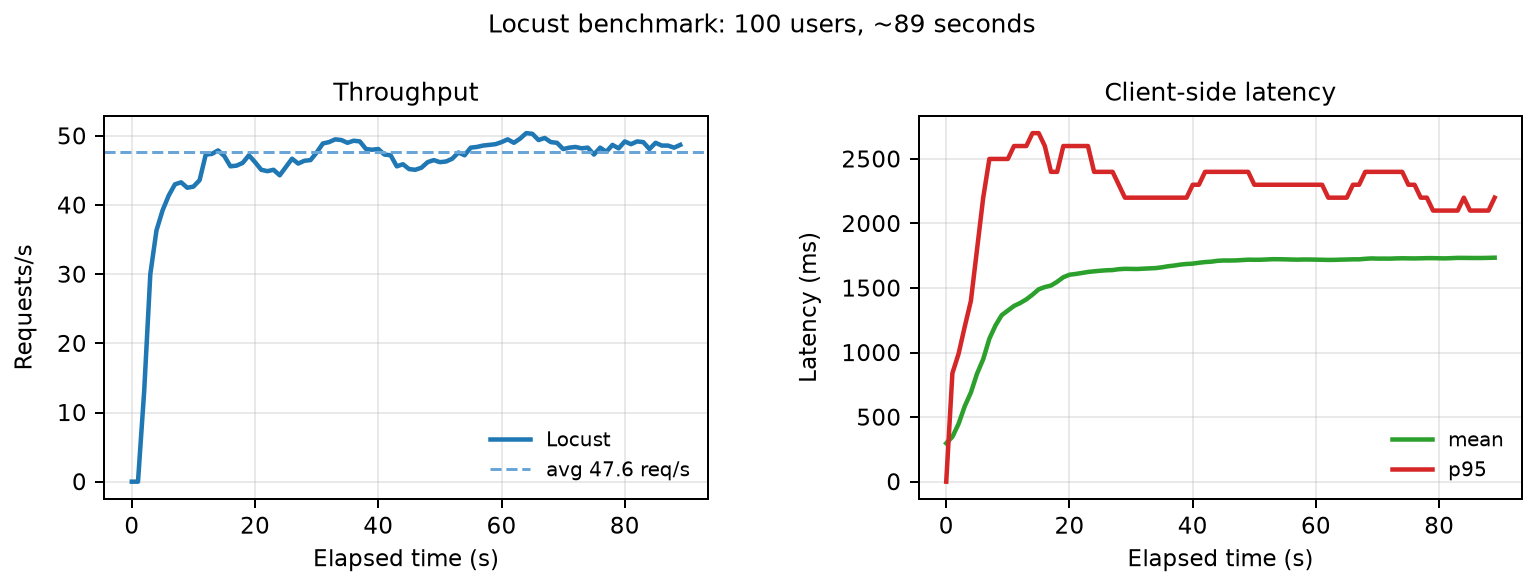
\includegraphics[width=0.8\linewidth]{assets/chart-locust-benchmark.png}
\caption{Bounded prototype serving replay: 100 Locust users, $\approx$89-second window.}
\label{fig:endpoint-benchmark}
\end{figure}

\section{Discussion}

The proposed framework reframes MLOps monitoring as part of an adaptive control loop: the model server emits production evidence, and the monitoring layer produces signals that can affect lifecycle decisions. This is useful for SaaS or PaaS-style settings where different users upload different models but need a common operational pipeline.

The scope is intentionally limited. First, the system targets tabular classification artifacts; image, text, time-series, and large language models need additional schema validation and monitoring metrics. Second, arbitrary user-uploaded artifacts introduce security risks, so hardened systems must isolate execution, validate dependencies, restrict archive extraction, and enforce resource quotas. Third, autonomous retraining and promotion require reliable evaluation gates, rollback policies, and human approval. Therefore, this baseline treats drift detection as an adaptation signal rather than an unconditional redeployment decision.

\section{Conclusion}

This paper presented a baseline drift-aware MLOps framework for multi-model serving, integrating tenant-aware onboarding, Kubernetes-native training, native model-evolution metadata, dynamic endpoints, asynchronous production logging, and reference-production drift monitoring. The system was formalized using tenants, model functions, production windows, drift indicators, lifecycle states, and adaptation actions, and instantiated with Network Intrusion Detection as a non-stationary security case study. Preliminary offline recovery results show that drift alerts can support review-driven challenger retraining on future holdout windows, while future work will address artifact-execution hardening, runtime deployment evidence, evaluation gates, and additional model types.

\begin{thebibliography}{00}

\bibitem{kreuzberger2023mlops}
M. Kreuzberger, N. Kuhl, and S. Hirschl, ``Machine Learning Operations (MLOps): Overview, Definition, and Architecture,'' \textit{IEEE Access}, vol. 11, pp. 31866--31879, 2023.

\bibitem{sculley2015debt}
D. Sculley, G. Holt, D. Golovin, E. Davydov, T. Phillips, D. Ebner,
V. Chaudhary, M. Young, J.-F. Crespo, and D. Dennison,
``Hidden Technical Debt in Machine Learning Systems,''
in \textit{Advances in Neural Information Processing Systems}, vol. 28, 2015.

\bibitem{amershi2019software}
S. Amershi, A. Begel, C. Bird, R. DeLine, H. Gall, E. Kamar,
N. Nagappan, B. Nushi, and T. Zimmermann,
``Software Engineering for Machine Learning: A Case Study,''
in \textit{Proc. IEEE/ACM 41st International Conference on Software Engineering:
Software Engineering in Practice}, 2019, pp. 291--300.

\bibitem{john2021towards}
M. M. John, H. H. Olsson, and J. Bosch, ``Towards MLOps: A Framework and Maturity Model,'' in \textit{Proc. 47th Euromicro Conference on Software Engineering and Advanced Applications}, 2021, pp. 1--8.

\bibitem{zhou2020pipeline}
Y. Zhou, Y. Yu, and B. Ding, ``Towards MLOps: A Case Study of ML Pipeline Platform,'' in \textit{Proc. International Conference on Artificial Intelligence and Computer Engineering}, 2020, pp. 494--500.

\bibitem{baylor2017tfx}
D. Baylor et al.,
``TFX: A TensorFlow-Based Production-Scale Machine Learning Platform,''
in \textit{Proc. 23rd ACM SIGKDD International Conference on Knowledge Discovery and Data Mining},
2017, pp. 1387--1395.

\bibitem{subramanya2022devops}
S. G. Subramanya, S. Shetty, V. Patil, S. K. Gad, and S. N. Bhat, ``From DevOps to MLOps: Overview and Application to Electricity Market Forecasting,'' \textit{Applied Sciences}, vol. 12, no. 19, 2022.

\bibitem{renggli2021data}
C. Renggli, B. Karlaš, B. Ding, F. Liu, K. Schawinski, W. Wu, and C. Zhang, ``A Data Quality-Driven View of MLOps,'' \textit{arXiv preprint arXiv:2102.07750}, 2021.

\bibitem{polyzotis2017data}
N. Polyzotis, S. Roy, S. E. Whang, and M. Zinkevich,
``Data Management Challenges in Production Machine Learning,''
in \textit{Proc. ACM International Conference on Management of Data}, 2017,
pp. 1723--1726.

\bibitem{gama2014survey}
J. Gama, I. Zliobaite, A. Bifet, M. Pechenizkiy, and A. Bouchachia, ``A Survey on Concept Drift Adaptation,'' \textit{ACM Computing Surveys}, vol. 46, no. 4, pp. 1--37, 2014.

\bibitem{webb2016drift}
G. I. Webb, R. Hyde, H. Cao, H.-L. Nguyen, and F. Petitjean,
``Characterizing Concept Drift,''
\textit{Data Mining and Knowledge Discovery}, vol. 30, no. 4,
pp. 964--994, 2016.

\bibitem{mlflow}
M. Zaharia et al., ``Accelerating the Machine Learning Lifecycle with MLflow,'' \textit{IEEE Data Engineering Bulletin}, vol. 41, no. 4, pp. 39--45, 2018.

\bibitem{crankshaw2017clipper}
D. Crankshaw, X. Wang, G. Zhou, M. J. Franklin, J. E. Gonzalez, and I. Stoica,
``Clipper: A Low-Latency Online Prediction Serving System,''
in \textit{Proc. 14th USENIX Symposium on Networked Systems Design and Implementation},
2017, pp. 613--627.

\bibitem{xgboost}
T. Chen and C. Guestrin, ``XGBoost: A Scalable Tree Boosting System,'' in \textit{Proc. 22nd ACM SIGKDD International Conference on Knowledge Discovery and Data Mining}, 2016, pp. 785--794.

\bibitem{cicids}
I. Sharafaldin, A. H. Lashkari, and A. A. Ghorbani, ``Toward Generating a New Intrusion Detection Dataset and Intrusion Traffic Characterization,'' in \textit{Proc. 4th International Conference on Information Systems Security and Privacy}, 2018, pp. 108--116.

\bibitem{sommer2010closedworld}
R. Sommer and V. Paxson,
``Outside the Closed World: On Using Machine Learning for Network Intrusion Detection,''
in \textit{Proc. IEEE Symposium on Security and Privacy}, 2010, pp. 305--316.

\bibitem{kubernetes}
B. Burns, B. Grant, D. Oppenheimer, E. Brewer, and J. Wilkes, ``Borg, Omega, and Kubernetes,'' \textit{Communications of the ACM}, vol. 59, no. 5, pp. 50--57, 2016.

\bibitem{Bhatt2025HarmonE}
H. Bhatt, S. Biswas, S. Rakhunathan, and K. Vaidhyanathan,
``HarmonE: A Self-Adaptive Approach to Architecting Sustainable MLOps,''
arXiv preprint arXiv:2505.13693, 2025. Accepted to ECSA 2025.
DOI: 10.48550/arXiv.2505.13693.

\bibitem{Zhang2025SSFNIDS}
X. Zhang, R. Zhao, Z. Jiang, H. Chen, Y. Ding, E. C. H. Ngai, and S.-H. Yang,
``Continual Learning with Strategic Selection and Forgetting for Network Intrusion Detection,''
arXiv preprint arXiv:2412.16264, 2025. Accepted by IEEE INFOCOM 2025.
DOI: 10.48550/arXiv.2412.16264.

\bibitem{MarcosMercade2026MLOpsFrameworks}
J. Marcos-Mercad\'e, U. Lopez-Novoa, and M. Ega\~na Aranguren,
``An Empirical Evaluation of Modern MLOps Frameworks,''
arXiv preprint arXiv:2601.20415, 2026.

\end{thebibliography}

\end{document}
